\documentclass[fontsize=11pt,reqno,a4paper,oneside]{scrartcl}

% ---- Sprache und Textformatierung ----
\usepackage{fontspec}
\usepackage{polyglossia}
\setdefaultlanguage{english}
\usepackage{microtype}
\usepackage{csquotes}
\usepackage{acronym}

% ---- KOMA-Script Seiteneinstellungen ----
\usepackage[onehalfspacing]{setspace}  
\usepackage[headsepline]{scrlayer-scrpage}
\usepackage{nowidow}

% Kopfzeilen-Konfiguration
\clearpairofpagestyles  % Alle bestehenden Kopf- und Fußzeilen löschen
\addtokomafont{pagehead}{\normalfont\small}  % Schriftart der Kopfzeile
\automark[section]{section}
\ihead{\textsc{\headmark}} 
\cfoot{\pagemark}

% ---- Mathematik und Symbole ----
\usepackage{amsmath, amsthm, amssymb, mathtools}
\usepackage[version=4]{mhchem}
\usepackage{chemformula}
\newcommand{\angstrom}{\text{\normalfont\AA}}

% ---- Graphische Pakete ----
\usepackage{xcolor}
\usepackage{graphicx}
\usepackage{float}
\usepackage{siunitx}
\usepackage{booktabs}
\usepackage{textpos}
\usepackage{subfig}
\usepackage{svg}
\usepackage{multirow}

% ---- Text-Positionierung ----
\usepackage[pscoord]{eso-pic}
\newcommand{\placetextbox}[3]{% \placetextbox{<horizontal pos>}{<vertical pos>}{<stuff>}
  \setbox0=\hbox{#3}% Put <stuff> in a box
  \AddToShipoutPictureFG*{% Add <stuff> to current page foreground
    \put(\LenToUnit{#1\paperwidth},\LenToUnit{#2\paperheight}){\vtop{{\null}\makebox[0pt][c]{#3}}}%
  }%
}%

% ---- Bibliographie ----
\usepackage[backend=biber,
    citestyle=numeric-comp,
    bibstyle=numeric,
    bibwarn=true,
    autocite=superscript,
    abbreviate=true, 
    sorting=none, 
    url=false, 
    doi=false,
    eprint=false,
    isbn=false]{biblatex}

% Definition eines neuen Zitierbefehls mit eckigen Klammern
\DeclareCiteCommand{\supercite}[\mkbibsuperscript]%
    {\usebibmacro{cite:init}%
        \let\multicitedelim\supercitedelim%
        \iffieldundef{prenote}%
        {}%
        {\BibliographyWarning{Ignoring prenote argument}}%
        \iffieldundef{postnote}%
        {}%
        {\BibliographyWarning{Ignoring postnote argument}}%
        \bibleftbracket}%
    {\usebibmacro{citeindex}%
        \usebibmacro{cite:comp}}
    {}%
    {\usebibmacro{cite:dump}%
        \bibrightbracket}

% Bibliographie-Dateien
\addbibresource{/Users/lucashirschfeld/sciebo/VsCode/LaTeX-Projects/bibliography/zotero.bib}

% ---- Hyperlinks ----
\usepackage{hyperref}
\hypersetup{colorlinks=true, linkcolor=black, citecolor=black, urlcolor=black}

% ---- Dokumenteinstellungen ----
\newcommand{\mylinespread}{1.5}
\setlength{\parindent}{0em}
\setlength{\parskip}{1em}

% ---- Metadaten ----
\def\Autor{Lucas Hirschfeld, s6luhirs@uni-bonn.de}
\def\Titel{\Acl{LEED} of the Au(111) surface and \acs{PTCDA} on the Au(111) surface}
\def\Date{First Submission: July 9, 2025 \\ Second Submission: \today}
\def\PiC{Supervisor: Morris Mühlpointner}
\def\Abstract{} 

\begin{document}
\pagestyle{empty}
\begin{titlepage}
    \begin{center}
        \vspace*{\fill}
        {\LARGE\bfseries \Titel}\par\vspace{2cm}
        {\Autor\par\vspace{0.5cm}\PiC\par\vspace{1cm}\par\vspace{0.2cm}\Date\par\vspace{5cm}}
    \end{center}
    {\Abstract\vspace{0.5cm}\par}\vfill
\end{titlepage}

\pagestyle{scrheadings}
\tableofcontents
\pagenumbering{arabic}
\clearpage

\section{Introduction}

\Acl{LEED} is a powerful and standard technique for investigating the surface structure of crystalline materials by the diffraction of low energy electrons. The technique was first used by Davisson and Germer in 1927 on a Nickel crystal.\autocite{Davisson1927} Since then, \ac{LEED} has become a widely used technique in surface science and materials research.\autocite{Kolasinski2012}

The basic principle of \ac{LEED} is to direct a beam of low-energy electrons onto a crystalline surface and to analyze the resulting diffraction pattern. The diffraction pattern is formed by the interference of the scattered electrons from the surface atoms, which leads to a characteristic pattern of bright spots on a fluorescent screen. The positions and intensities of these spots provide information about the surface structure, such as the lattice constant, surface reconstruction, and orientation of the surface.\autocite{Kolasinski2012}

The \ac{LEED} patterns formed by the scattered electrons show the reciprocal lattice of the surface and adsorbated structures. The reciprocal lattice vectors $\mathbf{a_j^*}$ and the real space lattice vectors $\mathbf{a_i}$ are related by the following equation:

\begin{equation}
\mathbf{a_i} \cdot \mathbf{a_j^*} = 2 \pi \delta_{ij},
\end{equation}

where $\delta_{ij}$ is the Kronecker delta, which is 1 if $i = j$ and 0 otherwise.

In this report, \ac{LEED} is used to investigate the surface structure of Au(111) and the adsorption of \ac{PTCDA} on this surface. The Au(111) surface is a well-studied model system in surface science due to its simple structure and well-defined surface properties.\autocite{Li2022,Dutta1963}

The Au(111) surface has a hexagonal close-packed structure with a lattice constant of approximately 2.88~\AA.\autocite{Dutta1963} The surface is known to undergo a (22x$\sqrt{3}$) reconstruction.\autocite{Li2022} 

The \ac{LEED} experiments in this report aim to determine the surface lattice constant, the bulk lattice constant, and the reconstruction of the Au(111) surface. Furthermore, the adsorption of \ac{PTCDA} on the Au(111) surface is investigated by measuring the \ac{LEED} pattern of \ac{PTCDA} on the Au(111) surface.

\clearpage
\section{Experimental}

\subsection{Experimental Setup}

The \ac{LEED} measurements were conducted in an \ac{UHV} chamber with a base pressure below $5 \cdot 10^{-10}$~\si{mbar}. The chamber was equipped with a turbomolecular pump and an ion getter pump. The sample was mounted on a sample holder that allowed for precise rotation and translation in all directions. As sample, a single crystal of Au(111) was used. The sample holder was equipped with a resistive heating element to facilitate annealing procedures and a thermocouple for temperature measurement.

Furthermore, the chamber was equipped with a \ac{LEED} optics system, which included an electron gun, a hemispherical fluorescent screen and a camera for recording the diffraction patterns.

\begin{figure}[htbp]
    \centering
    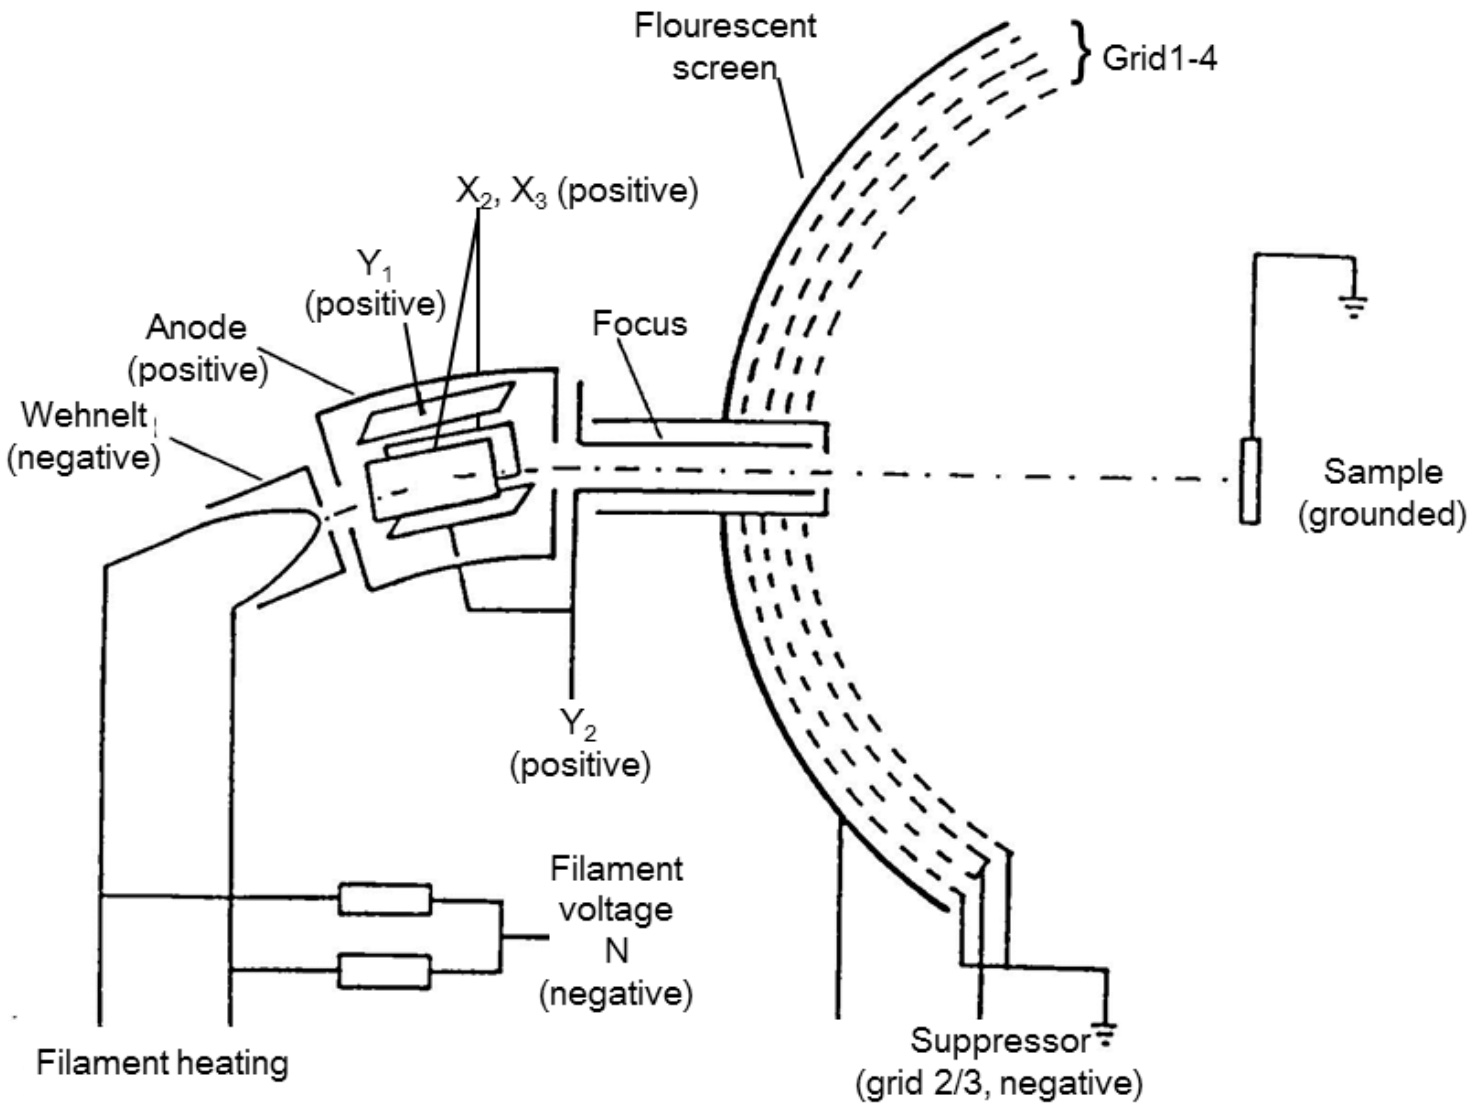
\includegraphics[width=0.8\textwidth]{images/experimental.jpg}
    \caption{Schematic (cross section) of the \ac{LEED} experimental setup including the individual voltages for the electron gun and the fluorescent screen. Taken from reference \cite{AKSokolowski2025}.}
    \label{fig:leed_setup}
\end{figure}

The \ac{LEED} optics has several components to generate and focus the electron beam onto the sample surface. The electron gun generates a beam of low-energy electrons, ranging from 50 to 200~\si{eV}, which is then focused by a series of lenses onto the sample surface. The electron beam is then scattered by the surface atoms, producing a diffraction pattern that is recorded by the fluorescent screen and camera. The parameters of the \ac{LEED} optics were optimized, using the provided interface on the computer, to achieve a high resolution and a low background noise.

\subsection{Sample Preparation}

The Au(111) single crystal surface was prepared in accordance with standard \ac{UHV} procedures. The Au(111) single crystal was subjected to an initial cleaning process involving the sputtering with Ar$^+$ ions with an energy of 1~\si{keV} for a duration of 30 minutes. This was followed by a subsequent annealing procedure at a temperature of 750~\si{K} for a period of 60 minutes. The cleaning procedure was executed at the onset of the experiment to guarantee a clean Au(111) surface for the \ac{LEED} measurements. Subsequently, the sample was then cooled down to room temperature, thus preparing it for the \ac{LEED} measurements.

After the \ac{LEED} measurements on the Au(111) surface, \ac{PTCDA} was evaporated onto the sample. Therefore, the evaporator was heated to a specific temperature and the sample was then rotated towards the evaporator to facilitate the deposition process.

\subsection{LEED Measurements}

\Ac{LEED} measurements were performed using the \ac{LEED} system explained before. The electron gun was operated at various energies between 25-200~\si{eV}. The filament heating was set to a constant current of 3.1 A. The electron beam was focused onto the sample surface, and the resulting diffraction pattern was depicted on the fluorescent screen. The diffraction patterns were captured using a camera, which allowed for high-resolution imaging of the diffraction spots.

With the optimized \ac{LEED} setup, several diffraction patterns were recorded at different electron energies and angles. First, the pure Au(111) surface was measured to obtain a reference pattern. Subsequently, the sample was rotated in steps of 5° to investigate the influence of the surface orientation on the diffraction pattern.

Afterwards, the diffraction pattern of the Au(111) surface was recorded at different electron energies, ranging from 80~\si{eV} to 200~\si{eV}. The diffraction patterns were analyzed to determine the spot distances and the lattice constant of the Au(111) surface. In addition, the reconstruction of the Au(111) surface was investigated by measuring the diffraction pattern at lower energies. The \ac{LEED} patterns from \autoref{sec:reconstruction} were analyzed to investigate the Au(111) surface reconstruction.

Finally, \ac{PTCDA} was deposited on the Au(111) surface by evaporation. The \ac{LEED} pattern of \ac{PTCDA} on the Au(111) surface was recorded at an electron energy of 23.4~\si{eV} to investigate the epitaxial growth of \ac{PTCDA} on the Au(111) surface.

\clearpage
\section{Results}

The results of the \ac{LEED} measurements are presented in the following sections. The first section discusses the orientation of the Au(111) surface in the diffraction pattern, followed by a section on the determination of the distance between the sample and the \ac{LEED} screen. Subsequently, the analysis of the \ac{LEED} pattern of the Au(111) surface is presented, including the determination of the lattice constant and the reconstruction of the Au(111) surface. Finally, the last section discusses the \ac{LEED} pattern of \ac{PTCDA} on the Au(111) surface.

\subsection{Orientation of the surface}

The orientation of the Au(111) surface in the diffraction pattern in comparison to a hard-sphere model was determined using the \ac{LEED} pattern obtained at an electron energy of 179.3~\si{eV}. The diffraction spots were analyzed by comparing the recorded diffraction pattern to the expected positions of the diffraction spots for a perfect Au(111) surface. \autoref{fig:surface_orientations} shows the surface orientation of the Au(111) crystal structure in comparison to the hard-sphere model.

\begin{figure}[htbp]
    \centering
    \subfloat[\ac{LEED} pattern of Au(111) at an energy of 179.3~\si{eV}]{
        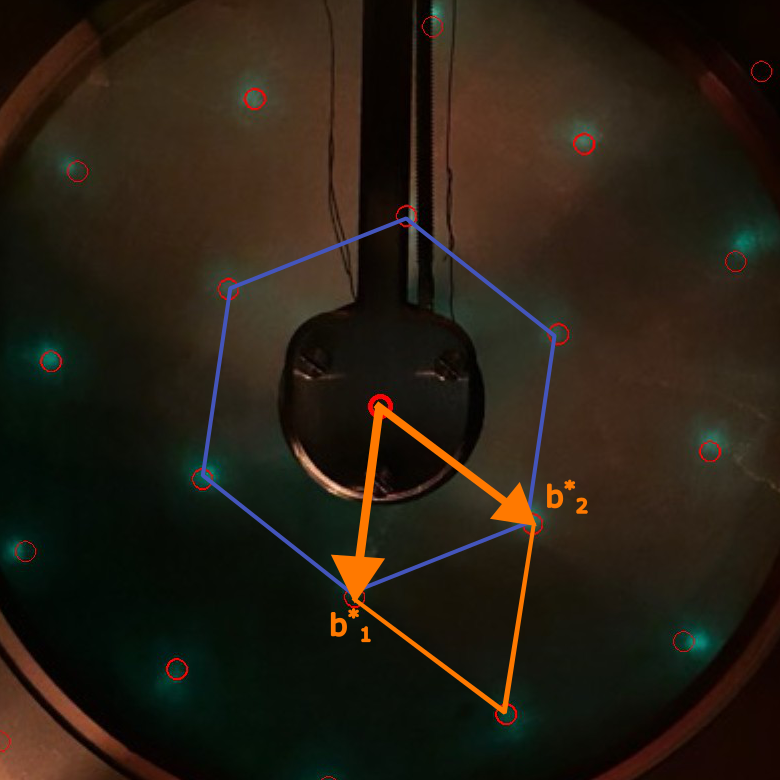
\includegraphics[width=0.47\textwidth]{images/image1-2.png}
        \label{fig:leed_orientation}
    }
    \hfill
    \subfloat[Hard-sphere model of the Au(111) surface]{
        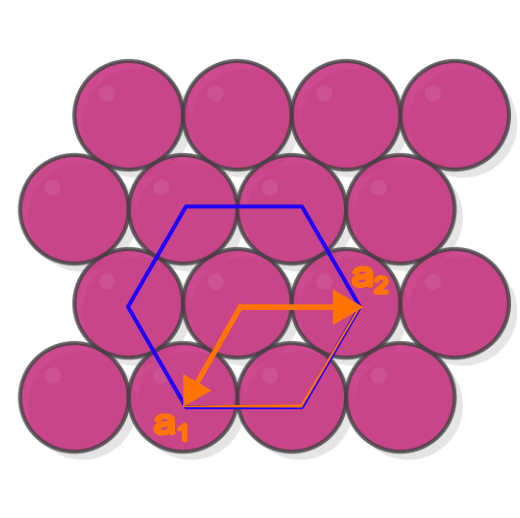
\includegraphics[width=0.47\textwidth]{images/surface-2.png}
        \label{fig:crystal_orientation}
    }
    
    \caption{Comparison of the \ac{LEED} pattern of the Au(111) surface at an electron energy of 179.3~\si{eV} with a hard-sphere model of the Au(111) surface. The red circles indicate the positions of the diffraction spots in the \ac{LEED} pattern. The blue hexagon shows the symmetry of the Au(111) surface. The orange vectors indicate the lattice vectors of the Au(111) surface. The orange lines show the unit cell.}
    \label{fig:surface_orientations}
\end{figure}

The diffraction spots in the \ac{LEED} pattern are arranged in a hexagonal pattern, which is consistent with the hard-sphere model of the Au(111) surface. Furthermore, it can be observed that the angle between the reciprocal lattice vectors of the Au(111) surface is approximately 60°, while the real space lattice vectors are at an angle of 120°. The reason for this difference is that the following relation holds for the reciprocal lattice vectors $\mathbf{b}$ and the real space lattice vectors $\mathbf{a}$:

\begin{equation}
\mathbf{a}_i \cdot \mathbf{b}_j = 2\pi \delta_{ij} ~\text{with}~\mathbf{a}_i \cdot \mathbf{b}_j= |\mathbf{a}_i| |\mathbf{b}_j| \cos(\psi).
\label{eq:lattice_vectors}
\end{equation}

\clearpage
\subsection{Determination of the sample distance to the LEED screen}

The spot distances in the \ac{LEED} pattern were measured to determine the distance $r$ between the Au(111) sample and the detector, which is equivalent to the \ac{LEED} screen radius. To fulfill this assumption, the sample has to be placed in the center of the sphere that is partly formed by the \ac{LEED} screen. The distances between the diffraction spots were extracted from the \ac{LEED} patterns in \autoref{fig:leed_patterns_angle} recorded at the same electron energy of 119.6~\si{eV} but at different angles.

\begin{figure}[htbp]
    \centering
    \subfloat[0° rotation]{
        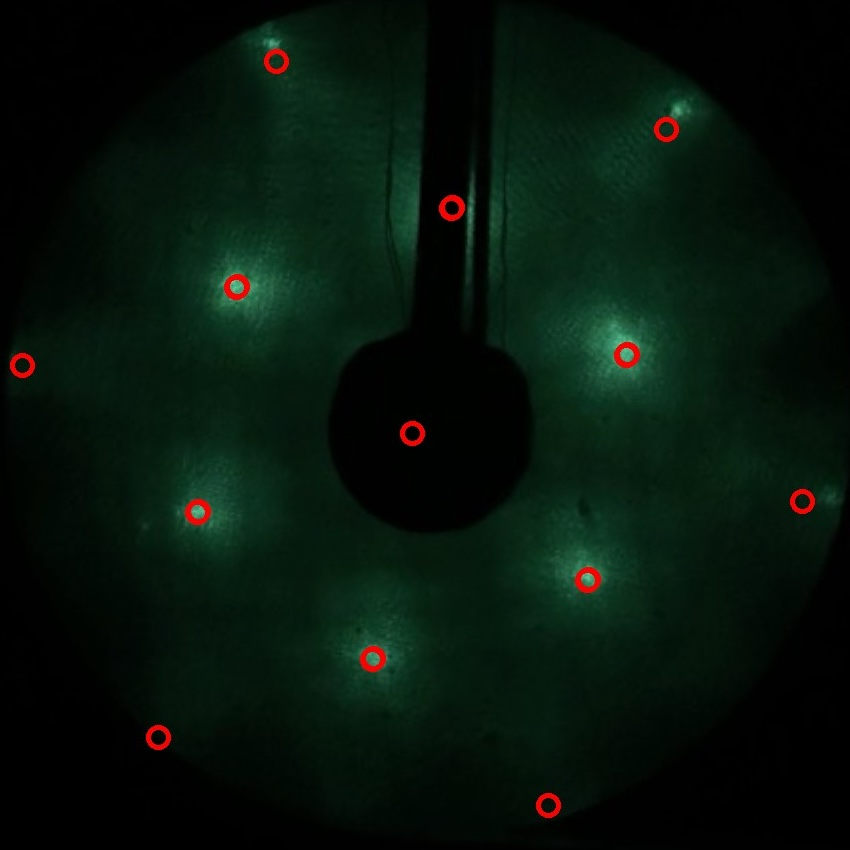
\includegraphics[width=0.47\textwidth]{images/119.6eV-1428-1054-1091-1310-1187-1219.jpg}
        \label{fig:leed_0deg}
    }
    \hfill
    \subfloat[5° rotation]{
        
\includegraphics[width=0.47\textwidth]{images/119.6ev-1428-1073-1094-1310-1197-1251-283Grad-1.jpg}
        \label{fig:leed_5deg}
    }
    
    \vspace{0.5cm}
    
    \subfloat[10° rotation]{
        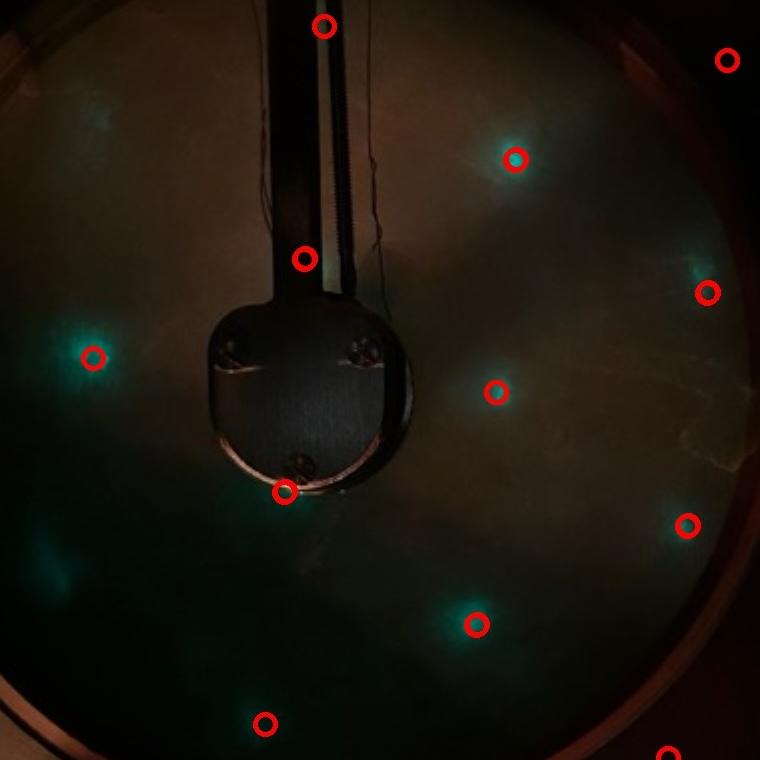
\includegraphics[width=0.47\textwidth]{images/119.6eV-1428-1073-1094-1310-1197-1251-288Grad.jpg}
        \label{fig:leed_10deg}
    }
    \hfill
    \subfloat[15° rotation]{
        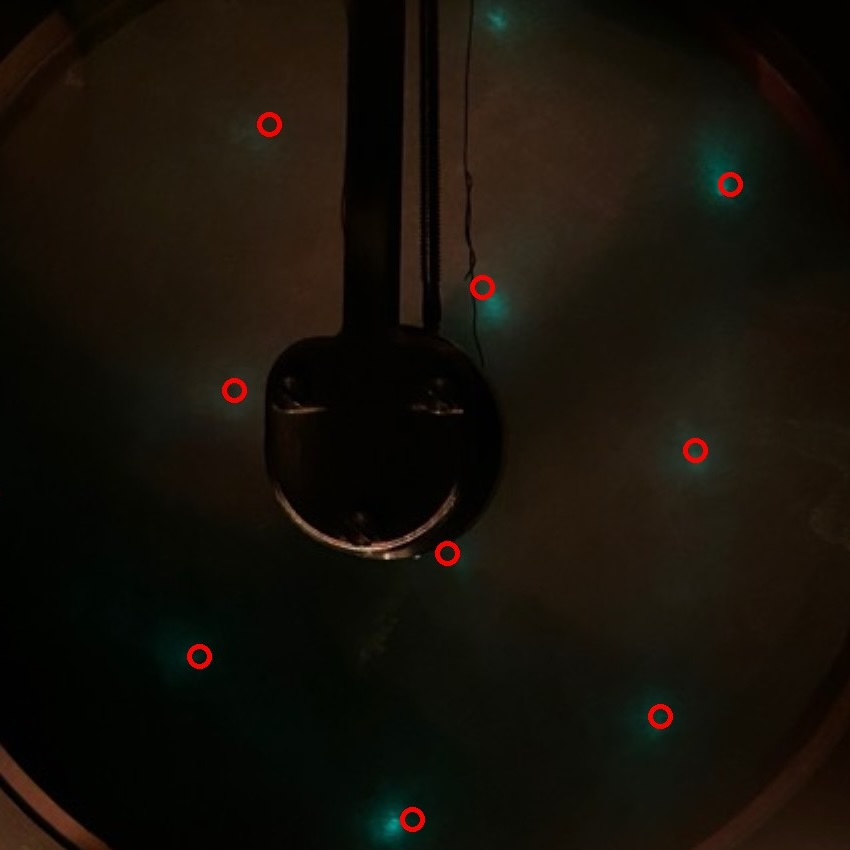
\includegraphics[width=0.47\textwidth]{images/120.5eV-1442-1085-1109-1326-1208-1262-293Grad.jpg}
        \label{fig:leed_15deg}
    }
    
    \caption{\ac{LEED} patterns of Au(111) surface at an electron energy of 119.6~\si{eV} and with different angles. The red circles indicate the positions of the diffraction spots.}
    \label{fig:leed_patterns_angle}
\end{figure}

The distances between the diffraction spots were measured in pixels and are summarized in \autoref{tab:spot_distances}. The distances were measured from the center of the diffraction pattern to the center of the diffraction spots, but only the projection in the radial direction was considered.

\begin{table}[htbp]
    \centering
    \caption{Measured distances between the diffraction spots in pixels for different angles.}
    \begin{tabular}{@{}cc@{}} \toprule
        angle $\theta$ (\si{\degree}) & distance $\Delta x$ [px] \\
        \midrule
        0 & 0 \\
        5 & 132 \\
        10 & 192 \\
        15 & 328  \\
        \bottomrule
    \end{tabular}
    \label{tab:spot_distances}
\end{table}

With the measured distances of the diffraction spots, the distance $r$ between the Au(111) sample and the \ac{LEED} screen can be determined using the formula:
\begin{equation}
    \sin(2 \theta) = \frac{\Delta x}{r},
    \label{eq:spot_distance}
\end{equation}
where $\Delta x$ is the distance between the diffraction spots in pixels and $\theta$ is the angle of the rotation.

Linearisation of equation \ref{eq:spot_distance} yields the distance $r$ by plotting $\sin(2\theta)$ against $\Delta x$. The slope of the linear fit to the data points gives the value of $1/r$. The resulting plot is shown in \autoref{fig:spot_distance_plot}.

\begin{figure}[htbp]
    \centering
    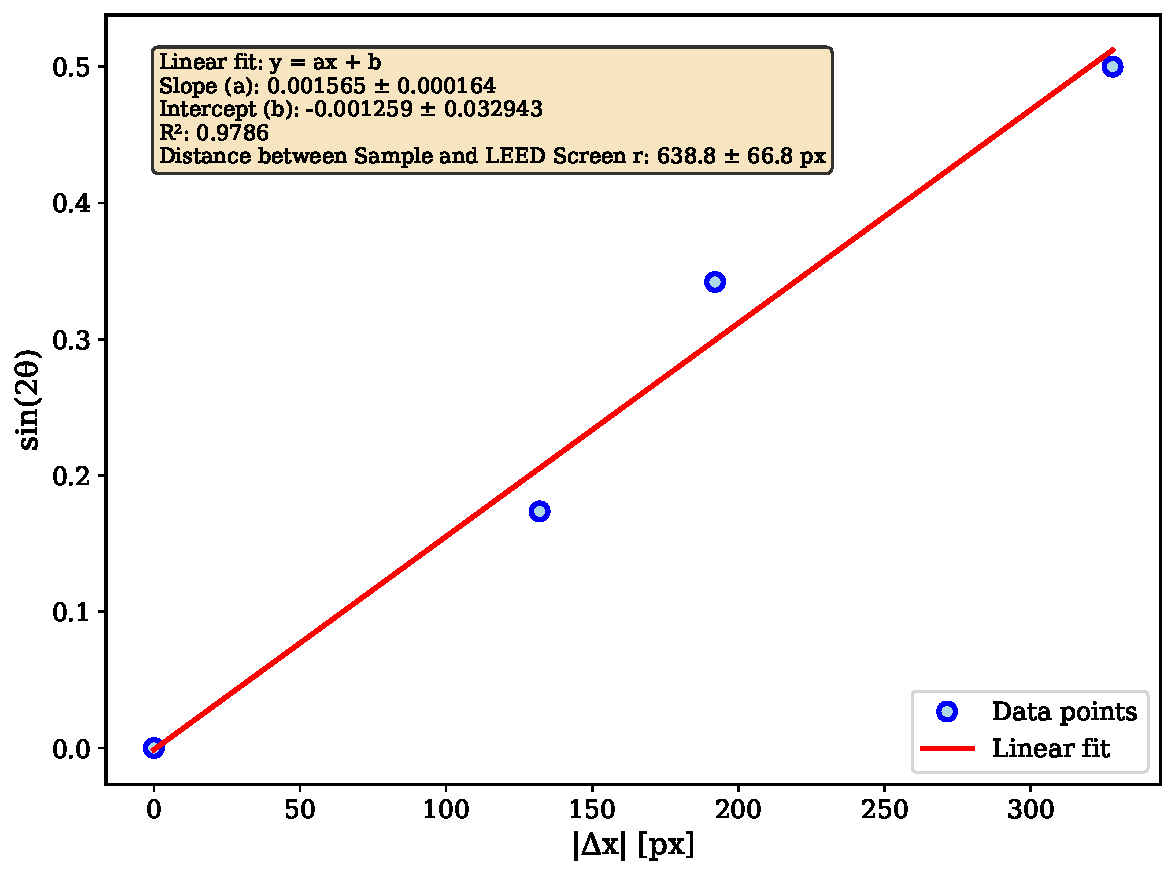
\includegraphics[width=0.8\textwidth]{images/LEED_sin2theta_vs_deltax.pdf}
    \caption{Plot of $\sin(2\theta)$ against the measured distances $\Delta x$ between the diffraction spots in pixels. The slope of the linear fit gives the value of $1/r$, where $r$ is the distance between the Au(111) sample and the detector.}
    \label{fig:spot_distance_plot}  
\end{figure}

The result of the linear fit is shown in \autoref{fig:spot_distance_plot}. The slope of the linear fit is $0.001565 \pm 0.000164$, which corresponds to a distance of $r = 638.8 \pm 66.8$~px between the Au(111) sample and the \ac{LEED} screen. The intercept of the linear fit is $-0.0001 \pm 0.0002$, which is more or less consistent with the expected value of zero, as the distance should be zero at an angle of zero.

\clearpage
\subsection{Determination of the lattice constant of the Au(111) surface}

The lattice constant of the Au(111) surface can be determined from the positions of the diffraction spots $d$ in the \ac{LEED} patterns and the distance between the sample and the \ac{LEED} screen $r$, which was determined from the linear fit in \autoref{fig:spot_distance_plot}. The distance between the spots $d$ is related to the lattice constant by the formula:

\begin{equation}
    \mathbf{a^*} = |\mathbf{a^*}| =  \frac{d}{r} |\mathbf{k_0}|,
    \label{eq:lattice_constant_reciprocal}
\end{equation}

where $\mathbf{a^*}$ is the reciprocal lattice vector, $d$ is the distance between the diffraction spots in pixels, $r$ is the distance between the sample and the \ac{LEED} screen in pixels and $|\mathbf{k_0}|$ is the wave vector of the electrons, which can be calculated from the electron energy $E$ using the formula:

\begin{equation}
    |\mathbf{k_0}| = \frac{2\pi}{\lambda_e} = \frac{2\pi}{\sqrt{\frac{h^2}{2m_e E}}},
    \label{eq:wave_vector}
\end{equation}

where $h$ is the Planck constant, $m_e$ is the electron mass and $E$ is the electron energy in \si{eV}. The wavelength $\lambda_e$ of the electrons can be calculated from the electron energy using the formula:

\begin{equation}
    \lambda_e = \frac{h}{\sqrt{2m_e E}}.
    \label{eq:wavelength}
\end{equation}

The wave vector $|\mathbf{k_0}|$ can be calculated for each electron energy used in the \ac{LEED} measurements.

\begin{figure}[htbp]
    \centering
    \subfloat[80.0~\si{eV}]{
        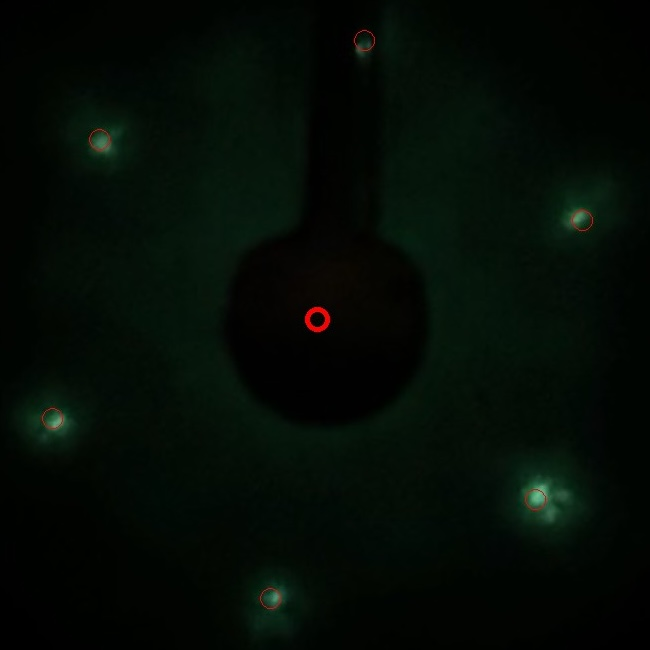
\includegraphics[width=0.47\textwidth]{images/80.0eV-858-719-828-831-718-490.jpg}
        \label{fig:leed_80eV}
    }
    \hfill
    \subfloat[120.0~\si{eV}]{
        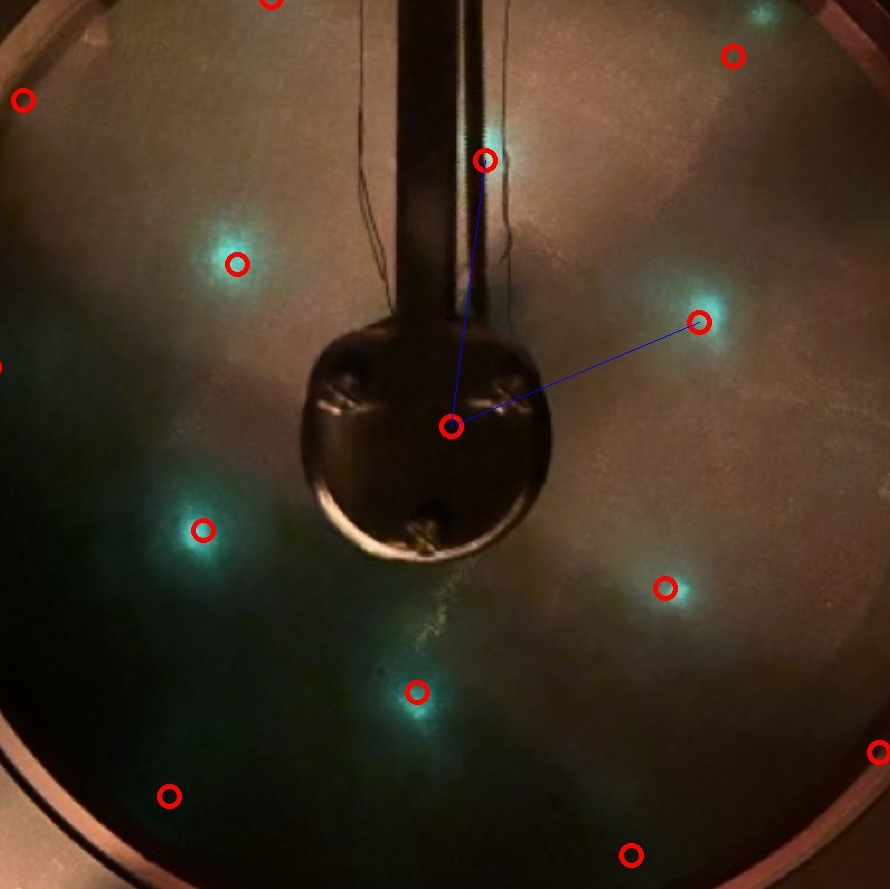
\includegraphics[width=0.47\textwidth]{images/120.0eV-1435-1156-1080-1321-1201-1010.jpg}
        \label{fig:leed_120eV}
    }
    
    \vspace{0.5cm}
    
    \subfloat[179.3~\si{eV}]{
        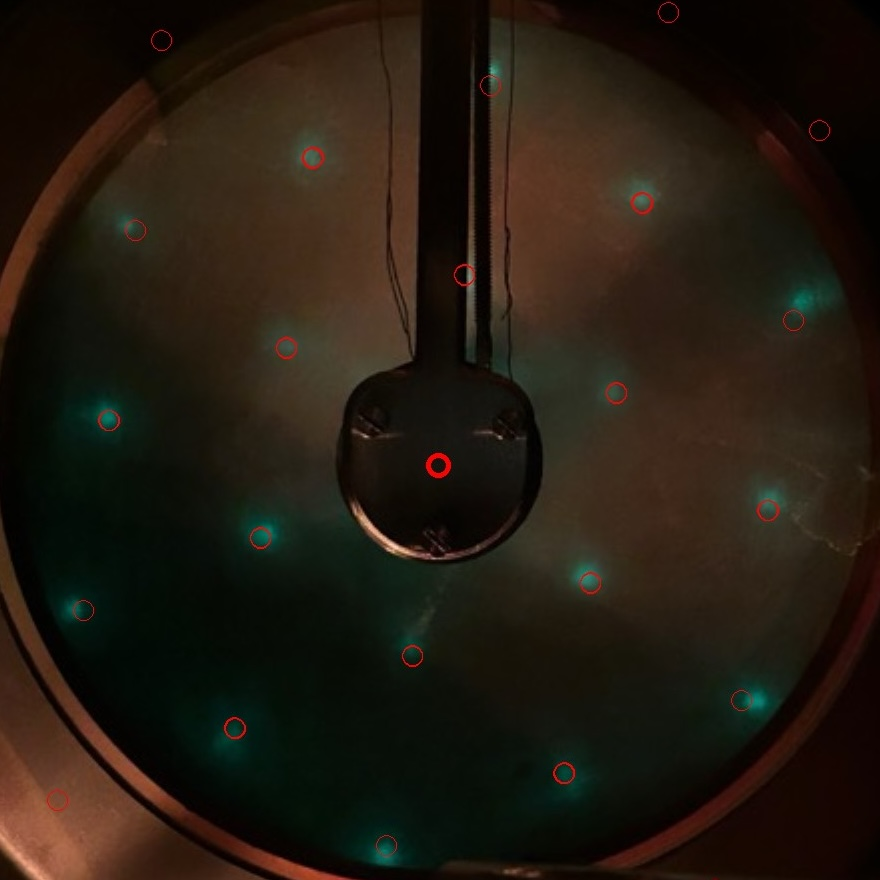
\includegraphics[width=0.47\textwidth]{images/179.3eV-2005-1740-2255-1883-1692-1849.jpg}
        \label{fig:leed_179eV}
    }
    \hfill
    \subfloat[198.7~\si{eV}]{
        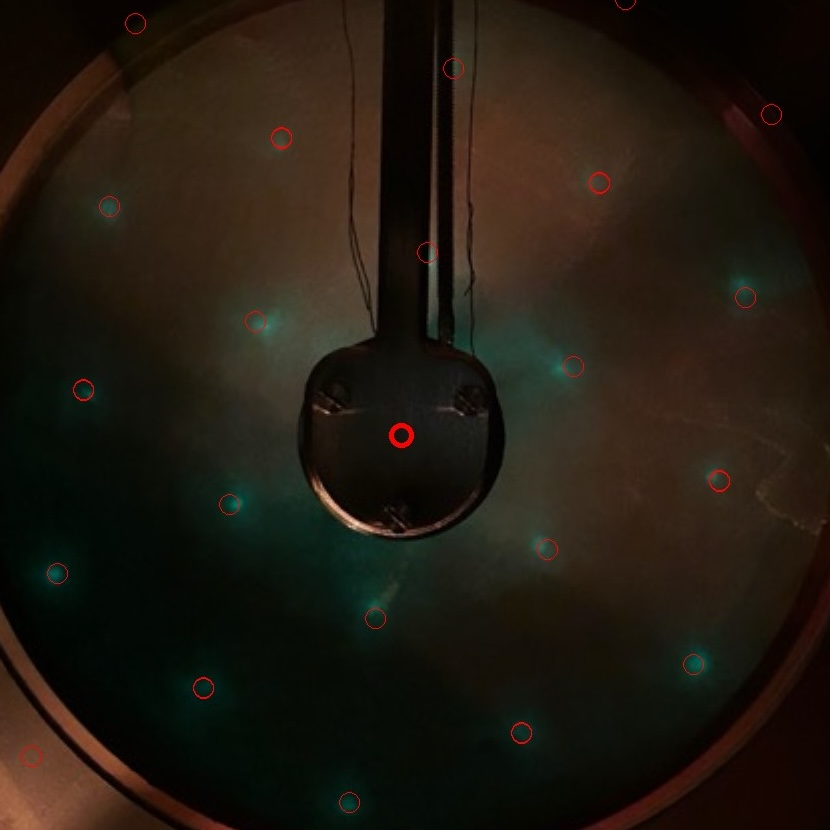
\includegraphics[width=0.47\textwidth]{images/198.7eV-2209-1887-2196-2268-1912-1786.jpg}
        \label{fig:leed_198eV}
    }
    
    \caption{LEED patterns of Au(111) surface at different electron energies showing the characteristic diffraction pattern. The red circles indicate the positions of the diffraction spots.}
    \label{fig:leed_patterns_energy}
\end{figure}

The \ac{LEED} patterns of the Au(111) surface at different electron energies are shown in \autoref{fig:leed_patterns_energy}. The distances between the diffraction spots were measured in pixels and are summarized in \autoref{tab:leed_lattice_parameters}. The distances were measured from the center of the diffraction pattern to the center of the diffraction spots. For each electron energy, the distances were measured for six different diffraction spots and the average distance was calculated. The average distance is shown in the last row of \autoref{tab:leed_lattice_parameters}.

With the measured distances of the diffraction spots $d$, the lattice constant in reciprocal space $a^*$ of the Au(111) surface can be determined using \autoref{eq:lattice_constant_reciprocal}. Using the reciprocal lattice vector $\mathbf{a^*}$, the surface lattice constant $\mathbf{a}$ in real space can be calculated using the formula:

\begin{equation}
    \mathbf{a} = |\mathbf{a}| = \frac{4\pi}{\sqrt{3}|\mathbf{a^*}|}.
    \label{eq:lattice_constant_real}
\end{equation}

The bulk lattice constant $\mathbf{a_b}$ can be calculated from the surface lattice constant $\mathbf{a}$ using the formula:

\begin{equation}
    \mathbf{a_b} = |\mathbf{a_b}| =  \sqrt{2} \cdot |\mathbf{a}|.
    \label{eq:lattice_constant_bulk}
\end{equation}

\begin{table}[htbp]
    \centering
    \caption{Measured \ac{LEED} spot distances and calculated lattice parameters for Au(111) surface at different electron energies.}
        \begin{tabular}{@{}ccccccc@{}} \toprule
                $E$ [eV] & $\lambda_e$ [\AA] & $\mathbf{k_0}$ [\AA$^{-1}$] & $d$ [pixel] & $\mathbf{a^*}$ [\AA$^{-1}$] & $\mathbf{a}$ [\AA] & $\mathbf{a_{b}}$ [\AA] \\
                \midrule
                \multirow{7}{*}{80.0} & \multirow{7}{*}{1.371} & \multirow{7}{*}{4.583} & 307.0 & $2.20 \pm 0.23$ & $3.29 \pm 0.35$ & $4.66 \pm 0.49$ \\
                & & & 310.5 & $2.23 \pm 0.23$ & $3.26 \pm 0.34$ & $4.61 \pm 0.48$ \\
                & & & 308.6 & $2.21 \pm 0.23$ & $3.28 \pm 0.34$ & $4.63 \pm 0.49$ \\
                & & & 308.2 & $2.21 \pm 0.23$ & $3.28 \pm 0.34$ & $4.64 \pm 0.49$ \\
                & & & 308.4 & $2.21 \pm 0.23$ & $3.28 \pm 0.34$ & $4.64 \pm 0.49$ \\
                & & & 306.9 & $2.20 \pm 0.23$ & $3.30 \pm 0.35$ & $4.66 \pm 0.49$ \\
                \cmidrule{4-7}
                & & & $308.3 \pm 1.4$ & $2.21 \pm 0.23$ & $3.28 \pm 0.34$ & $4.64 \pm 0.49$ \\
                \midrule \midrule
                \multirow{6}{*}{119.6} & \multirow{6}{*}{1.121} & \multirow{6}{*}{5.603} & 255.4 & $2.24 \pm 0.23$ & $3.24 \pm 0.34$ & $4.58 \pm 0.48$ \\
                & & & 253.7 & $2.23 \pm 0.23$ & $3.26 \pm 0.34$ & $4.61 \pm 0.48$ \\
                & & & 254.4 & $2.23 \pm 0.23$ & $3.25 \pm 0.34$ & $4.60 \pm 0.48$ \\
                & & & 251.6 & $2.21 \pm 0.23$ & $3.29 \pm 0.34$ & $4.65 \pm 0.49$ \\
                & & & 252.8 & $2.22 \pm 0.23$ & $3.27 \pm 0.34$ & $4.63 \pm 0.48$ \\
                & & & 253.5 & $2.22 \pm 0.23$ & $3.26 \pm 0.34$ & $4.61 \pm 0.48$ \\
                \cmidrule{4-7}
                & & & $253.6 \pm 1.4$ & $2.22 \pm 0.23$ & $3.26 \pm 0.34$ & $4.61 \pm 0.48$ \\
                \midrule \midrule
                \multirow{7}{*}{179.3} & \multirow{7}{*}{0.916} & \multirow{7}{*}{6.860} & 216.3 & $2.32 \pm 0.24$ & $3.12 \pm 0.33$ & $4.42 \pm 0.46$ \\
                & & & 219.4 & $2.36 \pm 0.25$ & $3.08 \pm 0.32$ & $4.35 \pm 0.46$ \\
                & & & 218.9 & $2.35 \pm 0.25$ & $3.09 \pm 0.32$ & $4.36 \pm 0.46$ \\
                & & & 215.2 & $2.31 \pm 0.24$ & $3.14 \pm 0.33$ & $4.44 \pm 0.46$ \\
                & & & 217.8 & $2.34 \pm 0.25$ & $3.10 \pm 0.32$ & $4.39 \pm 0.46$ \\
                & & & 217.1 & $2.33 \pm 0.24$ & $3.11 \pm 0.33$ & $4.40 \pm 0.46$ \\
                \cmidrule{4-7}
                & & & $217.4 \pm 1.6$ & $2.34 \pm 0.25$ & $3.11 \pm 0.33$ & $4.39 \pm 0.46$ \\
                \midrule \midrule
                \multirow{7}{*}{198.7} & \multirow{7}{*}{0.870} & \multirow{7}{*}{7.222} & 211.6 & $2.39 \pm 0.25$ & $3.03 \pm 0.32$ & $4.29 \pm 0.45$ \\
                & & & 213.6 & $2.42 \pm 0.25$ & $3.00 \pm 0.31$ & $4.25 \pm 0.44$ \\
                & & & 211.7 & $2.39 \pm 0.25$ & $3.03 \pm 0.32$ & $4.29 \pm 0.45$ \\
                & & & 210.0 & $2.37 \pm 0.25$ & $3.06 \pm 0.32$ & $4.32 \pm 0.45$ \\
                & & & 210.9 & $2.38 \pm 0.25$ & $3.04 \pm 0.32$ & $4.30 \pm 0.45$ \\
                & & & 209.0 & $2.36 \pm 0.25$ & $3.07 \pm 0.32$ & $4.34 \pm 0.45$ \\
                \midrule
                & & & $211.1 \pm 1.7$ & $2.39 \pm 0.25$ & $3.04 \pm 0.32$ & $4.30 \pm 0.45$ \\
                \bottomrule
            \end{tabular}
    \label{tab:leed_lattice_parameters}
\end{table}

\autoref{tab:leed_lattice_parameters} summarizes the measured distances between the diffraction spots $d$ in pixels, the calculated wave vector $|\mathbf{k_0}|$ in \AA$^{-1}$, the calculated reciprocal lattice constant $\mathbf{a^*}$ in \AA$^{-1}$, the calculated surface lattice constant $\mathbf{a}$ in \AA, and the calculated bulk lattice constant $\mathbf{a_b}$ in \AA~or the Au(111) surface at different electron energies. Furthermore, it is noteworthy that the obtained values for the electron energy of 80.0~\si{eV} and 119.6~\si{eV} are very similar larger than the values for the electron energies of 179.3~\si{eV} and 198.7~\si{eV}. This indicates that there is a systematic error in the measurements.

The final values for the reciprocal lattice constant, the surface lattice constant, and the bulk lattice constant of the Au(111) surface, averaged over all measured electron energies, are:

\begin{align*}
    \mathbf{a^*} &= 2.29 \pm 0.24~\text{\AA}^{-1} \\
    \mathbf{a}   &= 3.17 \pm 0.33~\text{\AA} \\
    \mathbf{a_b} &= 4.49 \pm 0.47~\text{\AA}
\end{align*}

These values are in agreement with the literature values for the Au(111) surface, which are 2.8810~\AA~for the surface lattice constant and 4.0743~\AA~for the bulk lattice constant\autocite{Dutta1963}.

\clearpage
\subsection{The reconstruction of the Au(111) surface}
\label{sec:reconstruction}

The reconstruction of the Au(111) surface was investigated by measuring the \ac{LEED} patterns with lower electron energies. The \ac{LEED} patterns of the Au(111) surface at two different electron energies are shown in \autoref{fig:reconstruction}. The blue circles indicate the positions of the substrate spots, while the red circles indicate the positions of the reconstruction spots.

\begin{figure}[htbp]
    \centering
    \subfloat[23.6~\si{eV}]{
        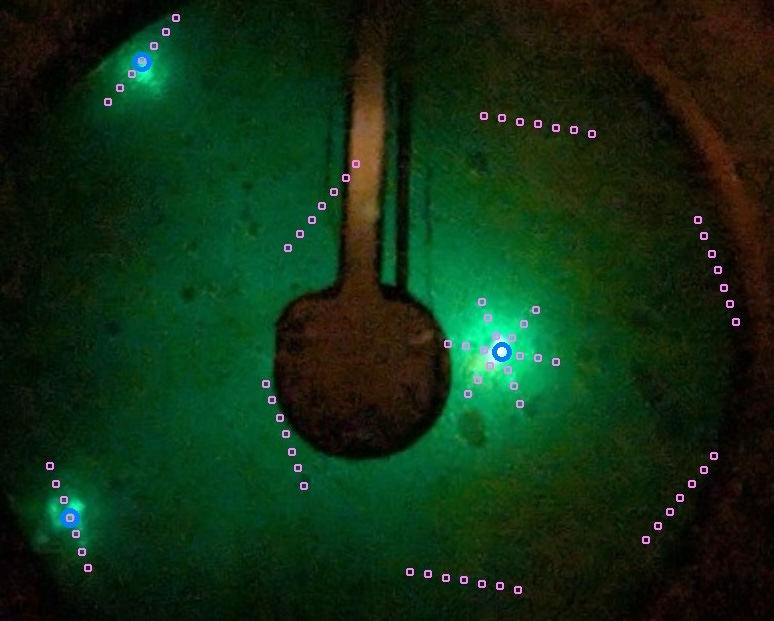
\includegraphics[width=0.47\textwidth]{images/R-23.6eV-320-204-334331-243-153-((22,0),(1,2)).jpg}
        \label{fig:reconstruction_23.4eV}
    }
    \hfill
    \subfloat[67.4~\si{eV}]{
        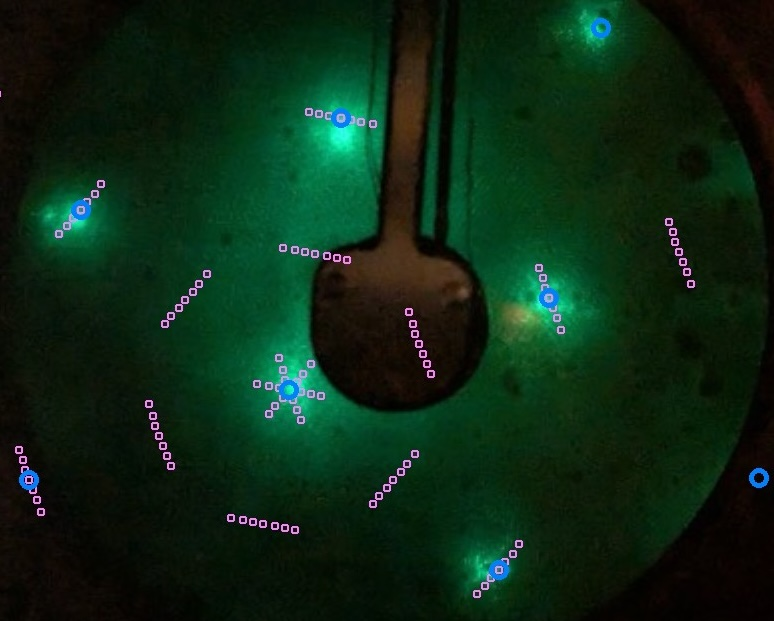
\includegraphics[width=0.47\textwidth]{images/R-67.4eV-821-646-846-927-691-417-((22,0),(1,2)).jpg}
        \label{fig:reconstruction_67.4eV}
    }

    \caption{\ac{LEED} patterns of the Au(111) surface at two different electron energies with the sample rotated showing the characteristic Au(111) reconstruction. The blue circles indicate the positions of the substrate spots. The reconstruction is indicated by the additional red circles in the pattern.}
    \label{fig:reconstruction}
\end{figure}

The reconstruction of the Au(111) surface can be observed in the \ac{LEED} patterns as additional diffraction spots that are not observed by unreconstructed surfaces. The additional diffraction spots are located at positions that are not consistent with the expected positions of the diffraction spots for a perfect fcc surface. 

The (22x$\sqrt{3}$) Au(111) surface reconstruction is a well-known phenomenon that occurs due to the relaxation of the surface atoms. The surface atoms are displaced from their ideal positions, resulting in a distortion of the surface lattice. This distortion leads to the formation of additional diffraction spots in the \ac{LEED} pattern.\autocite{Li2022}

The reconstruction of the Au(111) surface can be described by a (22x$\sqrt{3}$) superstructure, which is represented by the following superstructure matrix $\mathbf{M}$:

\begin{equation*}
    \mathbf{M} =
\begin{pmatrix}
22 & 0 \\
1 & 2
\end{pmatrix}.
\end{equation*} 

This superstructure matrix $\mathbf{M}$ is used to describe the positions of the additional diffraction spots in the \ac{LEED} pattern. The superstructure matrix is derived from the reciprocal lattice vectors of the Au(111) surface and the reconstruction.
\clearpage
\subsection{PTCDA on the Au(111) surface by epitaxial growth}

The growth of \ac{PTCDA} on the Au(111) surface was investigated using \ac{LEED}. The \ac{LEED} pattern of \ac{PTCDA} on the Au(111) surface shows a superstructure, indicating a long-range ordered arrangement of the molecules on the surface. The \ac{LEED} pattern of \ac{PTCDA} on the Au(111) surface at an electron energy of 23.4~\si{eV} is shown in \autoref{fig:ptcda}. The red circles indicate the positions of the center and the purple spots indicate the diffraction spots of the superstructure.

\begin{figure}[htbp]
    \centering
    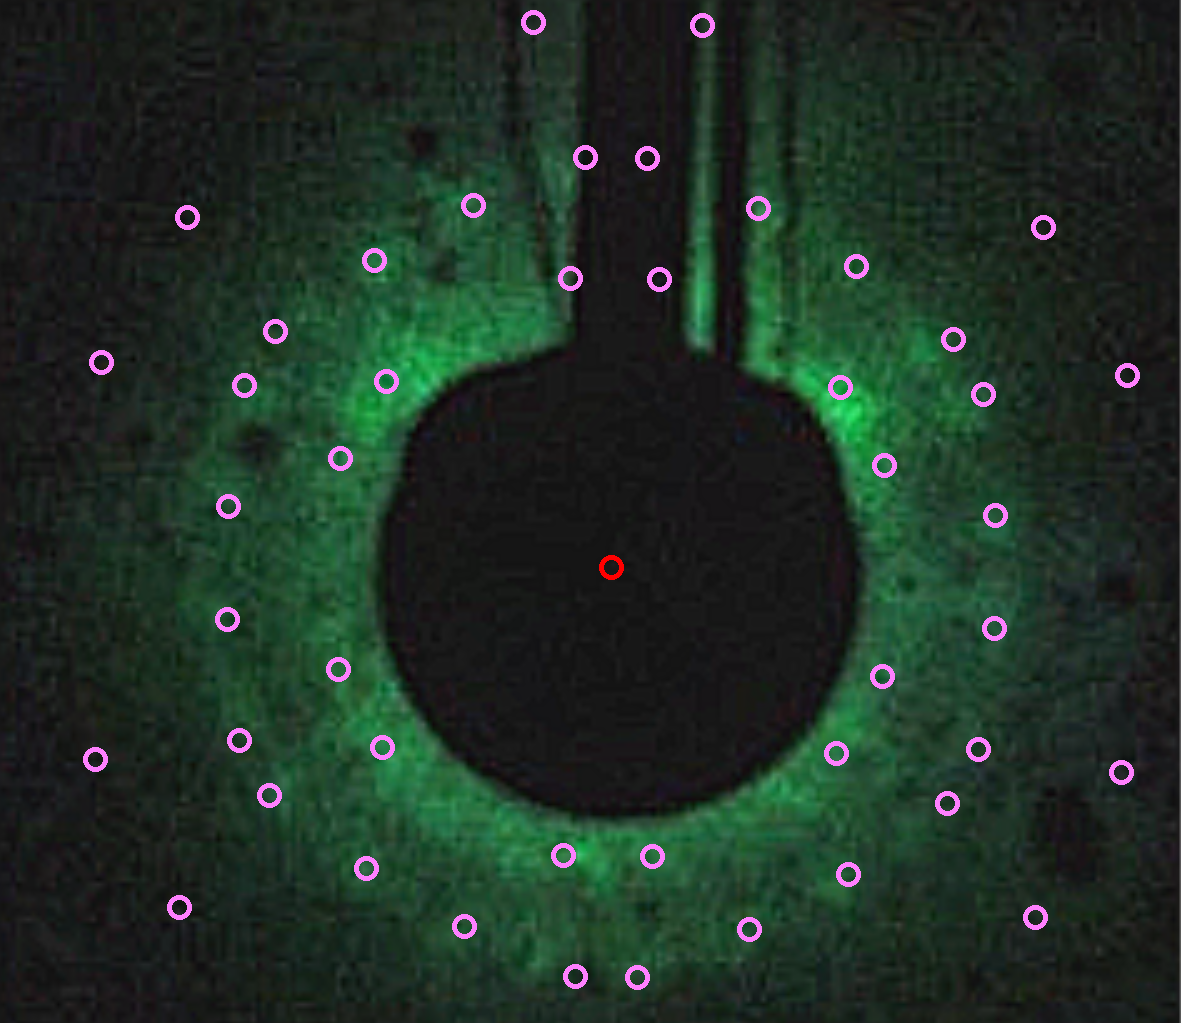
\includegraphics[width=0.47\textwidth]{images/23.4eV-327-329-311-316-233-231-2-((-0.92,4.66),(-7.87,-2.93)).jpg}
    \caption{\ac{LEED} pattern of \ac{PTCDA} on the Au(111) surface at an electron energy of 23.4~\si{eV}. The red circles indicate the positions of the center and the purple spots indicates the diffraction spots of the superstructure.}
    \label{fig:ptcda}
\end{figure}

The \ac{LEED} pattern of \ac{PTCDA} on the Au(111) surface shows a superstructure, which is consistent with the expected structure of \ac{PTCDA} on the Au(111) surface. The superstructure is characterized by an unit cell with different rotational domains, which is indicated by the additional diffraction spots in the \ac{LEED} pattern. The superstructure matrix $\mathbf{M}$ for the \ac{PTCDA} superstructure is given by:

\begin{equation*}
    \mathbf{M} =
\begin{pmatrix}
-0.92 & 4.66 \\
-7.82 & -2.93
\end{pmatrix}.
\end{equation*}

The superstructure matrix $\mathbf{M}$ from the literature\autocite{Kilian2002,Kilian2006} is used to describe the positions of the additional diffraction spots in the \ac{LEED} pattern. The superstructure matrix shows good agreement with the positions of the additional diffraction spots in the \ac{LEED} pattern of \ac{PTCDA} on the Au(111) surface. The superstructure matrix corresponds to an equilibrium structure of \ac{PTCDA} on the Au(111) surface, which is supported by the fact that the structure of the \ac{LEED} pattern was taken on a sample that was prepared two days before the picture was taken.


\clearpage
\section{Discussion}

\subsection{Determination of the lattice constant of the Au(111) surface}

The lattice constant of the Au(111) surface was determined from the \ac{LEED} pattern by analyzing the positions of the diffraction spots and the distance between the sample and the \ac{LEED} screen.

The obtained values for the surface lattice constant $\mathbf{a}$ and the bulk lattice constant $\mathbf{a_b}$ of the Au(111) surface are: $\mathbf{a} = 3.17\pm0.33$~\text{\AA}, and $\mathbf{a_b} = 4.49\pm0.47$~\text{\AA}.

The values are in agreement with the literature\autocite{Dutta1963}, which reports a surface lattice constant of 2.8810~\AA~and a bulk lattice constant of 4.0743~\AA. The difference between the obtained values and the literature values can be attributed to systematic errors in the measurements of distances, such as the determination of the distance between the sample and the \ac{LEED} screen and the distance of the diffraction spots to the center. 

\subsection{Reconstruction of the Au(111) surface}

The \ac{LEED} patterns of the Au(111) surface at different electron energies show the characteristic diffraction pattern of the (22x$\sqrt{3}$) reconstruction. Furthermore, the additional diffraction spots could be fitted with a superstructure matrix $\mathbf{M}$, which describes the positions of the additional diffraction spots in the \ac{LEED} pattern.

The superstructure matrix $\mathbf{M}$ for the (22x$\sqrt{3}$) reconstruction is given by:
\begin{equation*}
    \mathbf{M} =
\begin{pmatrix}
22 & 0 \\
1 & 2
\end{pmatrix}.
\end{equation*}

To conclude, the Au(111) surface reconstruction is observed in the \ac{LEED} experiments in this report and could be characterized by a (22x$\sqrt{3}$) superstructure. Nevertheless, \ac{LEED} measurements at not suitable for the determination of the unit cell for the reconstruction, as the diffraction spots are too close to each other and the resolution of the \ac{LEED} system is not sufficient to resolve the individual diffraction spots.


\subsection{PTCDA on the Au(111) surface}

The \ac{LEED} pattern of \ac{PTCDA} on the Au(111) surface shows a superstructure, which is consistent with the expected structure of \ac{PTCDA} on the Au(111) surface.\autocite{Kilian2002,Kilian2006} The superstructure is characterized by an unit cell with different rotational domains, which is indicated by the additional diffraction spots in the \ac{LEED} pattern. For a good description of all positions of the additional diffraction spots in the \ac{LEED} pattern, all rotational domains of the given superstructure matrix $\mathbf{M}$ must be used.

The superstructure matrix $\mathbf{M}$ for the \ac{PTCDA} superstructure is given by:
\begin{equation*}
    \mathbf{M} =
\begin{pmatrix}
-0.92 & 4.66 \\
-7.82 & -2.93
\end{pmatrix}
\end{equation*}

This superstructure matrix $\mathbf{M}$ corresponds to an possible superstructure matrix of the structure $\mathbf{B_1}$, which corresponds to an equilibrium structure of \ac{PTCDA} on the Au(111) surface.\autocite{Kilian2002,Kilian2006} The fact that it is an equilibrium structure is supported by the fact that the structure of the \ac{LEED} pattern was taken on a sample that was prepared two days before the picture was taken.

Furthermore, the superstructure matrix $\mathbf{M}$ indicates that the interactions between the \ac{PTCDA} molecules on the Au(111) surface are not strong enough to form a commensurate structure. This also shows that the interactions between different \ac{PTCDA} molecules are relevant for the formation of the superstructure on the Au(111) surface.


\clearpage
\section{Appendix}

\subsection*{Acronyms}

\begin{acronym}
    \acro{LEED}{low energy electron diffraction}
    \acro{PTCDA}{perylenetetracarboxylic dianhydride}
    \acro{UHV}{ultra-high vacuum}
\end{acronym}

\printbibliography[heading=bibintoc, title={References}] 

\end{document}